\section{Aufgabe 1-3}
Bei dieser Aufgabe werden vor allem Einstellungen gesucht, bei denen eine Aufnahme der Frank-Hertz-Kurve in möglichst schöner Form möglich sind. Dabei hängt das Aussehen der Kurve von verschiedenen Faktoren ab. Verwendet werden ein Funktionsgeneartor, der 
\begin{itemize}
\item[] \textbf{Heizspannung:} Da die Heizspannung für ein Austreten von Elektronen aus der Kathode sorgt, gibt es einen Zusammenhang zwischen dem Strom von Anode zu Gegenkathode \(I\) und der Heizspannung \(U_H\). Es ist eine genügend große Heizspannung zu wählen, um ein Austreten von Elektronen zu ermöglichen, ist diese erreicht hat eine weitere Erhöhung nur noch wenig Effekt, sorgt im Allgemeinen aber für eine Erhöhung des Stroms \(I\).
\item[] \textbf{Beschleunigungsspannung:} Die Beschleunigungsspannunng ist die Spannung \(U_B\), die zweischen Anode und Kathode angelegt wird. Sie sorgt dafür, dass sich die Elektronen in einem Elektrischen Feld befinden und somit \textit{beschleunigt} werden.

Bei diesem Versuchsaufbau wird die Beschleunigungsspannung variiert, indem eine Wechselspannung verwendet wird.
\item[] \textbf{Temperatur:} Die Temperatur wird bei dem Vorhandenen Versuchsaufbau eingestellt, indem ein Thermostat an der Apparatur selbst eingestellt wird, der eine elektrische Heizung steuert. Da der Thermostat sehr langsam reagiert ist die Temperatur nur schwer genau einstellbar und ändert sich selbst während einer Messung erheblich.

Sie sorgt dafür, dass das Quecksilber in den gasförmigen Zustand übergeht, da sonst kein ausreichender Abstand der Atome gegeben ist.
\end{itemize}
\subsection{Aufbau}
Der Aufbau wurde schon fertig vorgefunden. Es werden daher nur alle Steckverbindungen auf deren Richtigkeit überprüft und die Geräte eingeschaltet und der Computer für die Aufnahme der Messwerte hochgefahren. Verwendet werden die Franck-Hertz-Röhre mit Heizthermostat und Heizung, ein USB-Oszilloskop für den Computer und ein speziell für den Franck-Hertz-versuch gefertigtes Netzteil für die Spannungsversorgung der Apparatur. Anschließend wird mit der Durchführung begonnen.
\subsection{Durchführung}
Im Rahmen der ersten Aufgabe wurde zunächst eine Einstellung gesucht, bei der im X-Y-Bild ein möglichst gut erkennbarer Kurvenverlauf sichtbar wurde. Angezeigt wurde \(I\) über \(U_B\), wobei \(I\) nicht exakt gemessen wurde sondern nur eine proportionale Spannung über einen Widerstand detektiert wurde. Aufgrund eines Hinweises des leitenden Tutors wurde dahingehend von der Aufgabenstellung abgewichen, dass Kurven für \(155, 185, 205\, ^\circ C\) aufgenommen wurden, da diese leichter zu messen sind.
\subsection{Fehlerbetrachtung}
Die Fehler der Messung ist im Allgemeinen nur schwer anzugeben, daher werden die Fehler der Steigungen aus der Streuung berechnet. Das USB-Oszilloskop hat eine begrenzte Auflösung, was man an der Rasterstruktur der Messwerte sehen kann, außerdem streuen die Messwerte auch erheblich, was an den breiten Kurven zu sehen ist. Des weiteren sind auch diverse systematische Fehler vorhanden gewesen, z.B. wurde um die Spannung zu messen ein Spannungsteiler verwendet, der den Messwert weiter verfälscht.
\subsection{Graphen/Messwerte}
Die Messdaten wurden als Textdatei aus dem Programm exportiert und anschließend mit GNU-Plot dargestellt dabei wurde der Faktor 10 für die echte Spannung für \(U_B\) berücksichtigt. Die Minima wurden nur mit Augenmaß geschätzt, da ein Kurven-\textit{fitting} aufgrund der  breiten Streuung der Messwerte nicht möglich war. 
\begin{center}
\begin{minipage}{\linewidth}
\centering
\makebox[0cm]{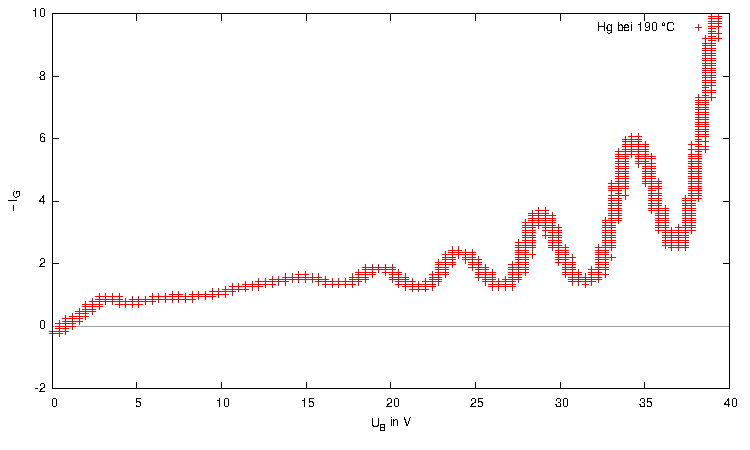
\includegraphics[width=\textwidth]{graphen/a1/a1}}
\captionof{figure}{Erste für A2 aufgenommene Franck-Hertz-Kurve (\(T=190\,^\circ C\))}
\label{a1}
\end{minipage}
\begin{minipage}{\linewidth}
\centering
\makebox[0cm]{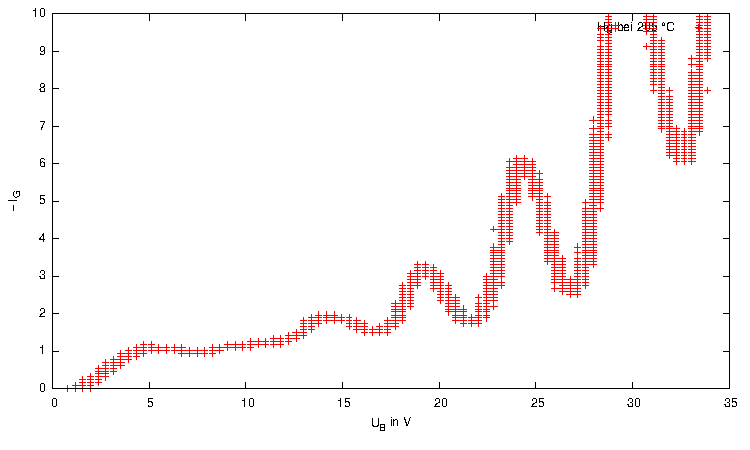
\includegraphics[width=\textwidth]{graphen/a2/a2c}}
\captionof{figure}{Erste für A3 aufgenommene Franck-Hertz-Kurve (\(T=155\,^\circ C\))}
\label{a2a}
\end{minipage}
\begin{minipage}{\linewidth}
\centering
\makebox[0cm]{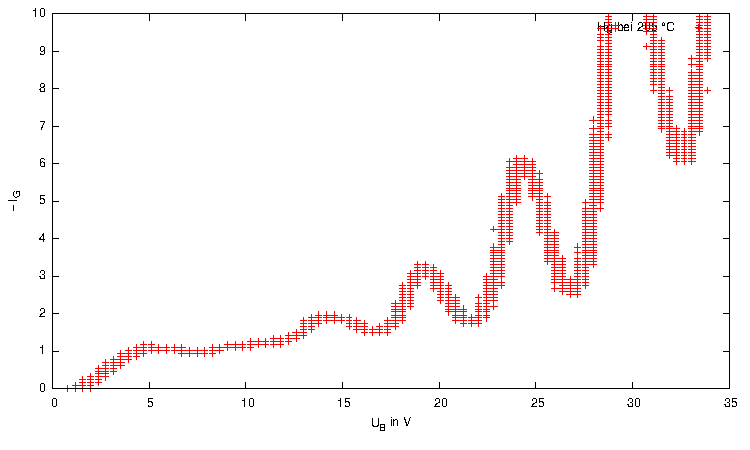
\includegraphics[width=\textwidth]{graphen/a2/a2c}}
\captionof{figure}{Erste für A3 aufgenommene Franck-Hertz-Kurve (\(T=185\,^\circ C\))}
\label{a2b}
\end{minipage}
\begin{minipage}{\linewidth}
\centering
\makebox[0cm]{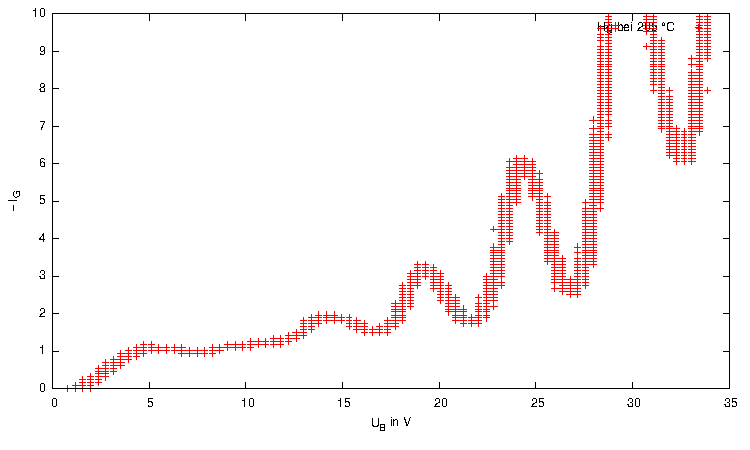
\includegraphics[width=\textwidth]{graphen/a2/a2c}}
\captionof{figure}{Erste für A3 aufgenommene Franck-Hertz-Kurve (\(T=205\,^\circ C\))}
\label{a2c}
\end{minipage}
\end{center}
Die so gefunden Spannungen \(U_B\) der Minima werden nun tabelliert und anschließend mit einer linearen regression dargestellt um die Steigung \(b\) des als linear angenommen Verlaufs zu erhalten.
\begin{center}
\begin{tabular}{c|c|c|c|c}
Minimum & \(T=190\,^\circ C\) & \(T=155\,^\circ C\) & \( T=185\,^\circ C\) & \(T=205\,^\circ C\)\\\hline
\(0\) & \(11,85\, V\) & \(11,85\, V\) & \(11,85\, V\) & \(11,85\, V\)\\
\(1\) & \(21,90\, V\) & \(11,85\, V\) & \(11,85\, V\) & \(11,85\, V\)\\
\(2\) & \(26,65\, V\) & \(11,85\, V\) & \(11,85\, V\) & \(11,85\, V\)\\
\(3\) & \(31,50\, V\) & \(11,85\, V\) & \(11,85\, V\) & \(11,85\, V\)\\
\(4\) & \(36,85\, V\) & \(11,85\, V\) & \(11,85\, V\) & \(11,85\, V\)\\
\end{tabular}
\captionof{table}{Minima von \(U_B\) der aufgenommenen Franck-Hertz-Kurven}
\end{center} 
\subsection{Auswertung}
\subsection{Fazit}